\begin{figure}[h]

% \begin{equation*}
%   \textcolor{blue}{\lambda x} . (\textcolor{red}{\lambda y} . (\lambda z . \textcolor{red}{y}) \textcolor{red}{y}) \textcolor{blue}{x}
% \end{equation*}
%
% \begin{equation*}
%   \textcolor{blue}{\lambda}\ (\textcolor{red}{\lambda}\ (\lambda\ \textcolor{red}{1})\ \textcolor{red}{0})\ \textcolor{blue}{0}
% \end{equation*}

\centering
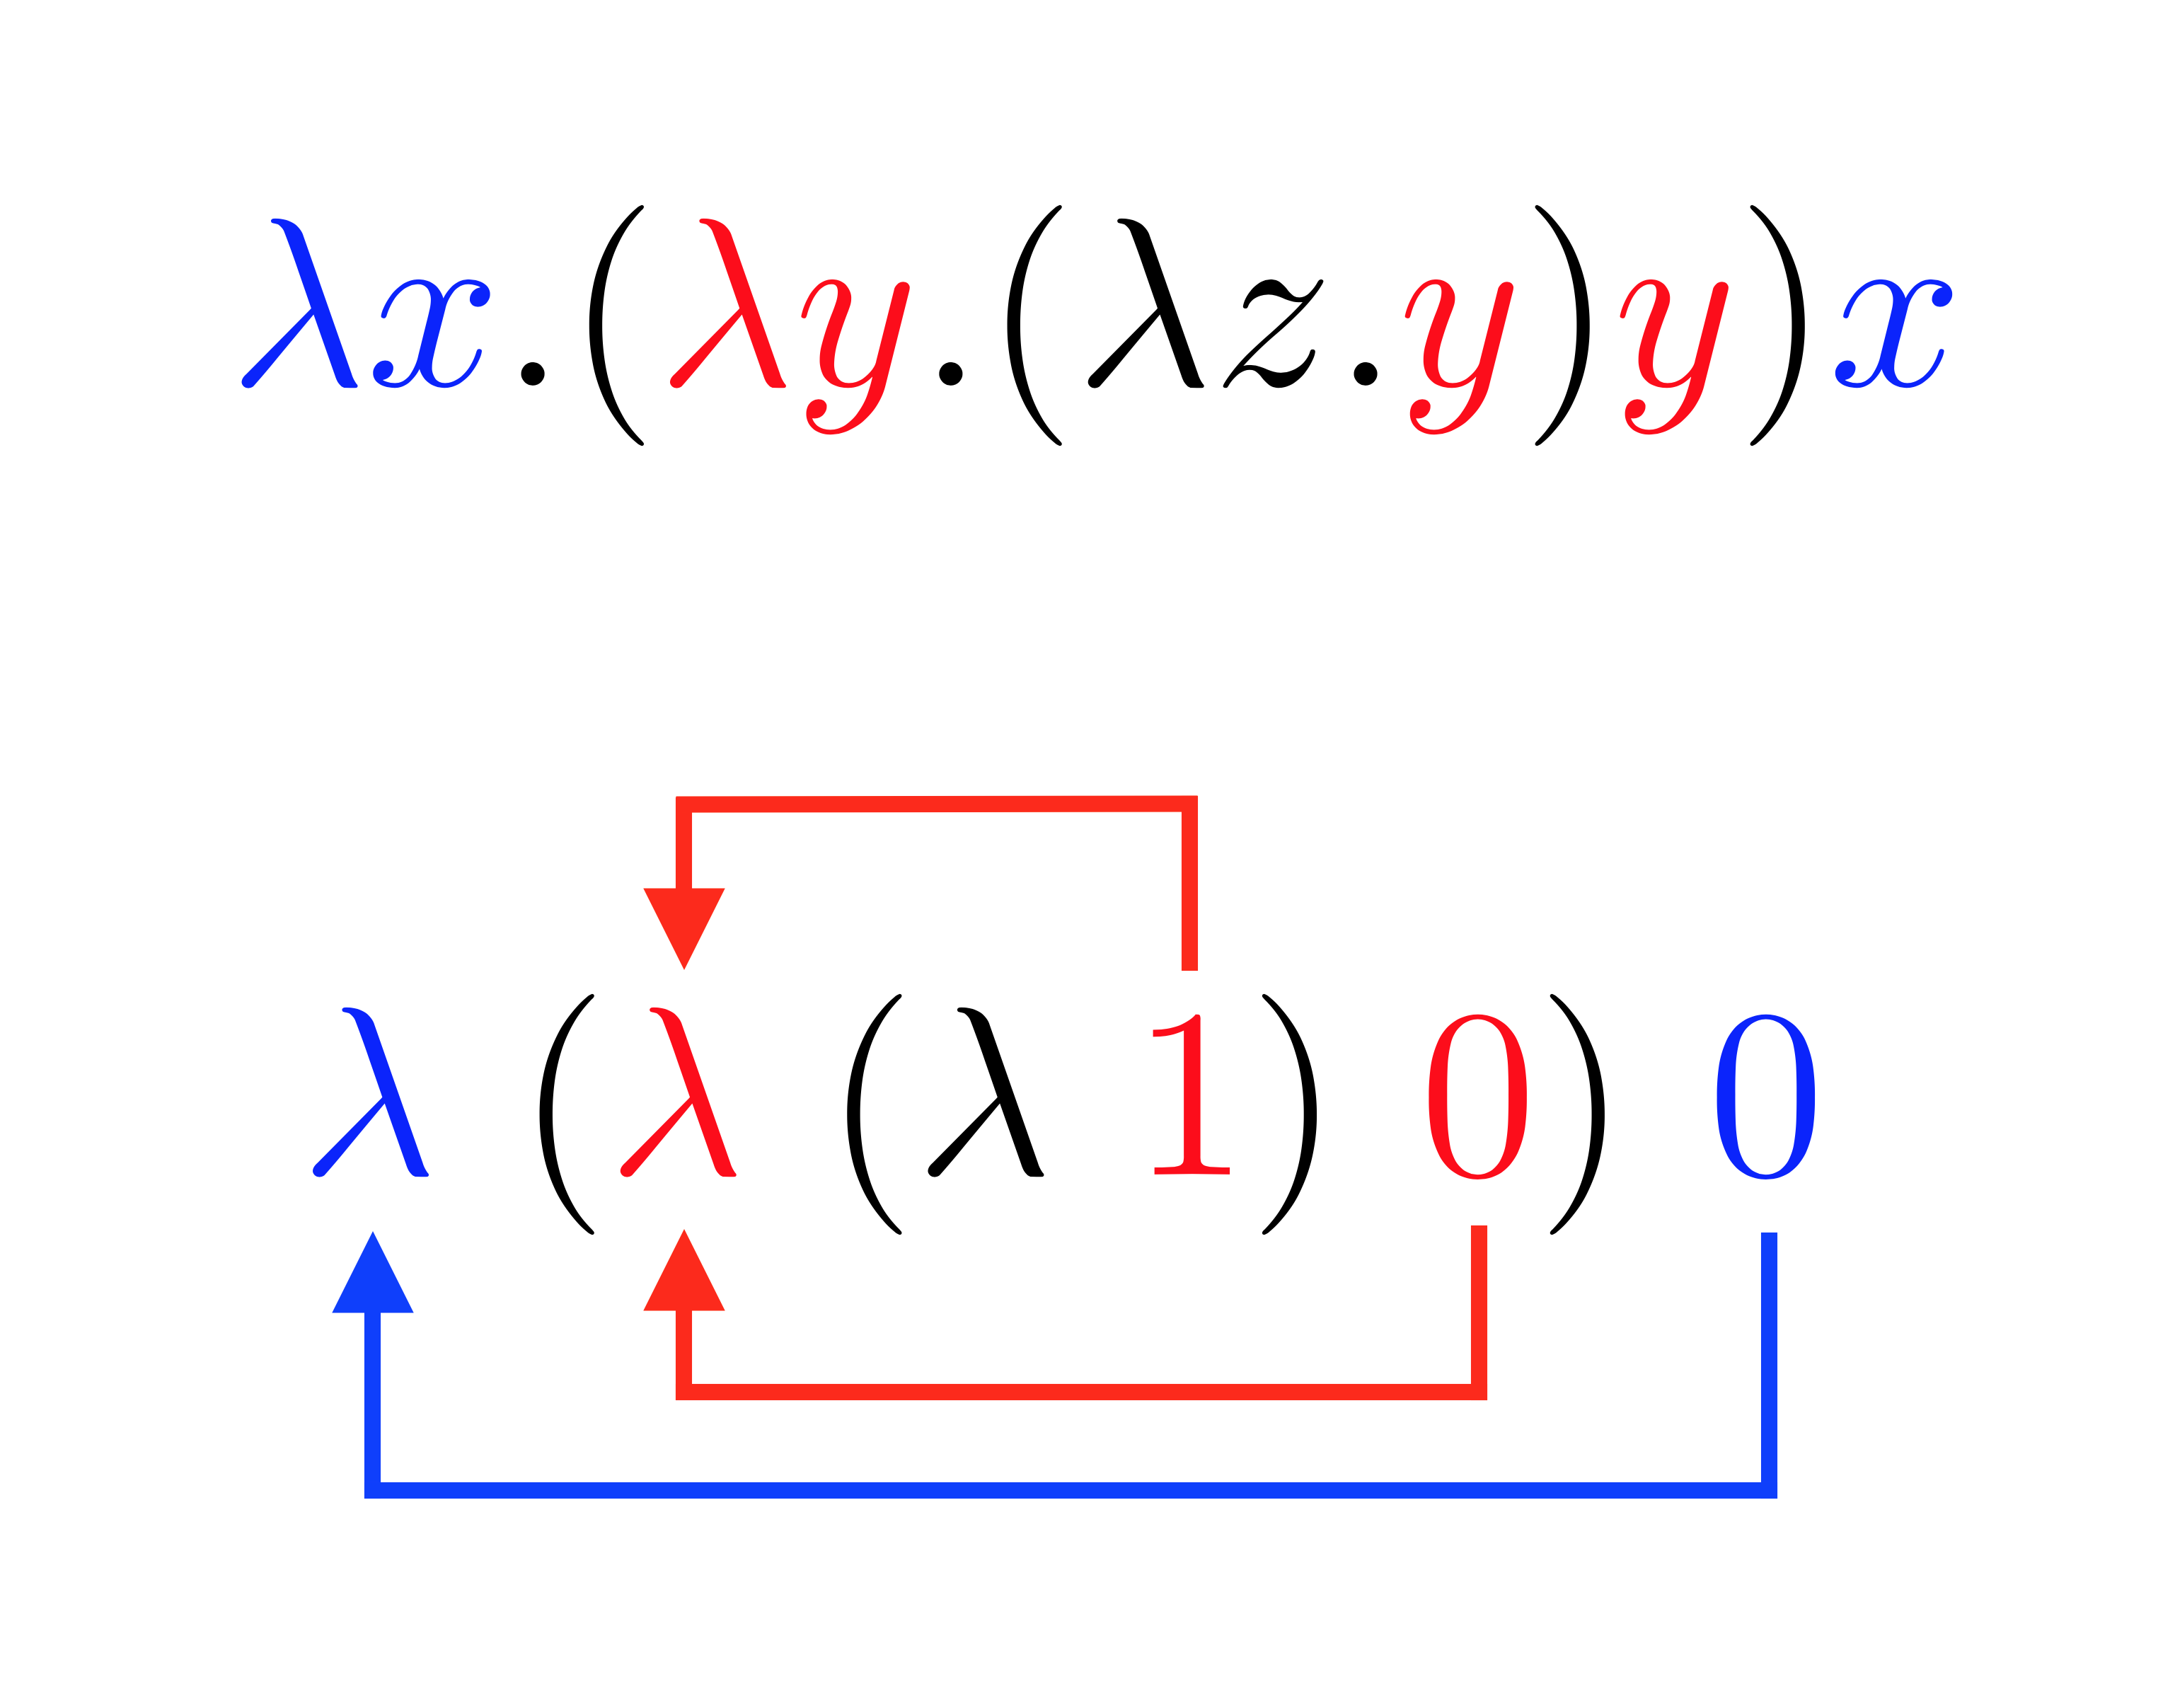
\includegraphics[width=4cm]{Figures/DeBruijnIndex}

\caption{An example of a (circumlocutious) identity function as a de Bruijn indexed $\lambda$-calculus expression.}
\label{fig:db_example}
\end{figure}
